\clearpage\begingroup
\HistoricalHead{182}{L}{PHYSIK.\quad NACHLASS.}
\newcommand{\AbsoluteMaasseFigureFour}{%
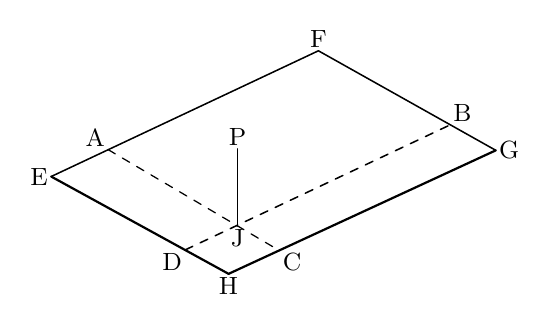
\begin{tikzpicture}[x=.0095cm,y=-.0095cm,line cap=round,line join=round,every node/.style={font=\small,inner sep=1pt}]
\coordinate (E) at (34,219);
\coordinate (F) at (391,51);
\coordinate (G) at (628,184);
\coordinate (H) at (271,349);
\coordinate (A) at (110,183);
\coordinate (B) at (567,150);
\coordinate (C) at (339,318);
\coordinate (D) at (213,317);
\coordinate (J) at (283,285);
\coordinate (P) at (283,182);
\draw[line width=.55pt] (E)--(F)--(G);
\draw[line width=.8pt] (G)--(H)--(E);
\draw[line width=.45pt,dash pattern=on 3pt off 3pt] (A)--(C);
\draw[line width=.55pt,dash pattern=on 3pt off 3pt] (D)--(B);
\draw[line width=.5pt] (J)--(P);
\node[left] at (E) {E};
\node[above] at (F) {F};
\node[right] at (G) {G};
\node[below] at (H) {H};
\node[above left] at (A) {A};
\node[above right] at (B) {B};
\node[below right] at (C) {C};
\node[below left] at (D) {D};
\node[below] at (J) {J};
\node[above] at (P) {P};
\end{tikzpicture}}

\begin{center}5.\end{center}
\noindent\hspace*{\parindent}Wir wollen jetzt die Wirkung eines Stromes, der die vier Seiten eines Rechtecks $EFGH$ durchläuft, auf einen Punkt $P$ bestimmen. Es sei $PJ=k$ das Perpendikel aus $P$ auf die Ebene des Rechtecks und $AC$ und $DB$[*)] mit den Seitenpaaren des Rechtecks parallel. Wir bezeichnen $AP,BP,CP,DP$ mit $a,b,c,d$; $AJ,BJ,CJ,DJ$ mit $\alpha,\beta,\gamma,\delta$, für den Fall der Figur als positiv betrachtet; endlich $EP,FP,GP,HP$ mit $e,f,g,h$, so dass
\begin{center}\AbsoluteMaasseFigureFour\par\small Figur 4.\end{center}
\[
\begin{gathered}
aa=\alpha\alpha+kk,\quad bb=\beta\beta+kk,\quad cc=\gamma\gamma+kk,\quad dd=\delta\delta+kk,\\
ee=\alpha\alpha+\delta\delta+kk=aa+\delta\delta=dd+\alpha\alpha\text{ u. s. w.}
\end{gathered}
\]

\clearpage\SourceLeaf{188}\HistoricalHead{183}{R}{WECHSELWIRKUNGEN ZWISCHEN GALVANISCHEN STRÖMEN UND MAGNETISMUS.}
Fiele $J$ ausserhalb des Rechtecks, so würde nur eine oder einige der Grössen $\alpha,\beta,\gamma,\delta$ negativ zu setzen sein.

Dem vorigen Artikel zufolge ist die Wirkung von $EF$ auf $P$
\[
=\frac{\beta}{af}+\frac{\delta}{ae}.
\]
\noindent Die Richtung dieser Kraft ist normal gegen $AP$, und insofern der Strom in der Richtung $EFGH$ geht und das Rechteck horizontal gedacht wird, nach unten zu gerichtet; sie zerlegt sich in Eine senkrecht gegen die Ebene des Rechtecks
\[
=\frac{\alpha\beta}{aaf}+\frac{\delta\alpha}{aae}
\]
\noindent und eine parallel mit $AC$
\[
=\frac{k\beta}{aaf}+\frac{k\delta}{aae}.
\]
\noindent Behandelt man ebenso die drei anderen Seiten, so findet man, dass die ganze auf $P$ wirkende Kraft sich in folgende drei zerlegt:

I. Normal gegen das Planum, nach unten zu
\par\medskip\noindent
\begin{minipage}[c]{.57\linewidth}
\[
\begin{aligned}
&\frac{\delta\alpha}{dde}+\frac{\delta\alpha}{aae}\\[4pt]
&+\frac{\alpha\beta}{aaf}+\frac{\alpha\beta}{bbf}\\[4pt]
&+\frac{\beta\gamma}{bbg}+\frac{\beta\gamma}{ccg}\\[4pt]
&+\frac{\gamma\delta}{cch}+\frac{\gamma\delta}{ddh}
\end{aligned}
\]
\end{minipage}\hfill
\begin{minipage}[c]{.39\linewidth}
Man bemerkt leicht, dass diese acht Theile die Wirkung der acht Stücke des Stroms $DE,EA,AF,FB,BG,GC,CH,HD$ ausdrücken.
\end{minipage}\par\medskip

II. Parallel mit $AC$
\[
\frac{k\beta}{aaf}+\frac{k\delta}{aae}-\frac{k\delta}{cch}-\frac{k\beta}{ccg}.
\]

III. Parallel mit $BD$
\[
\frac{k\alpha}{bbf}+\frac{k\gamma}{bbg}-\frac{k\gamma}{ddh}-\frac{k\alpha}{dde}.
\]
\noindent Die Formeln werden einfacher, wenn $J$ in der Mitte von $AC$ oder $BD$[*)] liegt. Im ersten Falle wird\begingroup\renewcommand{\thefootnote}{}\footnotetext{[*) Hier Schreibfehler der Handschrift.]}\endgroup
\[
\begin{aligned}
a&=c,\quad e=h\\
\alpha&=\gamma,\quad f=g,
\end{aligned}
\]
\clearpage\SourceLeaf{189}\HistoricalHead{184}{L}{PHYSIK.\quad NACHLASS.}
\noindent Also die Kraft I
\[
=2\left(\frac{\alpha\delta}{aae}+\frac{\alpha\delta}{dde}+\frac{\alpha\beta}{aaf}+\frac{\alpha\beta}{bbf}\right),
\]
\noindent die Kraft $\mathrm{II}=0$,\par\noindent die Kraft III
\[
=2\left(\frac{k\alpha}{bbf}-\frac{k\alpha}{dde}\right).
\]
\noindent Liegt $J$ in der Mitte des Rechtecks, so dass zugleich $\alpha=\gamma$, $\beta=\delta$, folglich $a=c$, $b=d$, $e=f=g=h$, so wird die Kraft I
\[
=4\left(\frac{\alpha\beta}{aae}+\frac{\alpha\beta}{bbe}\right)
\]
\noindent und sowohl die Kraft II als $\mathrm{III}=0$.
\clearpage\endgroup
